%\subsection{Observations and motivation} % just find the proble and benefit
%\label{sec:background}
%
%\subsection{Need of Deduplication}
%
%In order to understand the extent of storage requirements and performance demands from a Docker registry. 
%We observe the amount of public repositories hosted by Docker Hub registries. 
%The number of public repositories is constantly increasing with a growth that amounts 
%to around one million repositories annually. 
%This corresponds to~130\,TB of annual growth in storage requirements (but it is acually less because of shared layers, right?), 
%costing around~\$15,000 a month if Google Cloud Storage is used~\cite{GoogleCloudStoragePricing}.
%This growth implies significant benefits to storage deduplication. 
%
%Deduplication option, block level, file level ...?
%
%
%
%\paragraph{Deduplication statistics} % the potiential of deduplication 
%
%how dedup will help
%
%
%layer ref count 
%
%\paragraph{Deduplication ratio growth} % benefit

\subsection{Need for User Behavior based Cache Management}

%\paragraph{Access skewness}
%According to ~\cite{dockerworkload}, 
%\paragraph{Reuse time distribution}
%\subsubsection{Observations}

%\paragraph{Layers that belong to the same repo have different popularity}
\begin{figure}[t]
	\centering
		\begin{minipage}{0.225\textwidth}
			\centering
			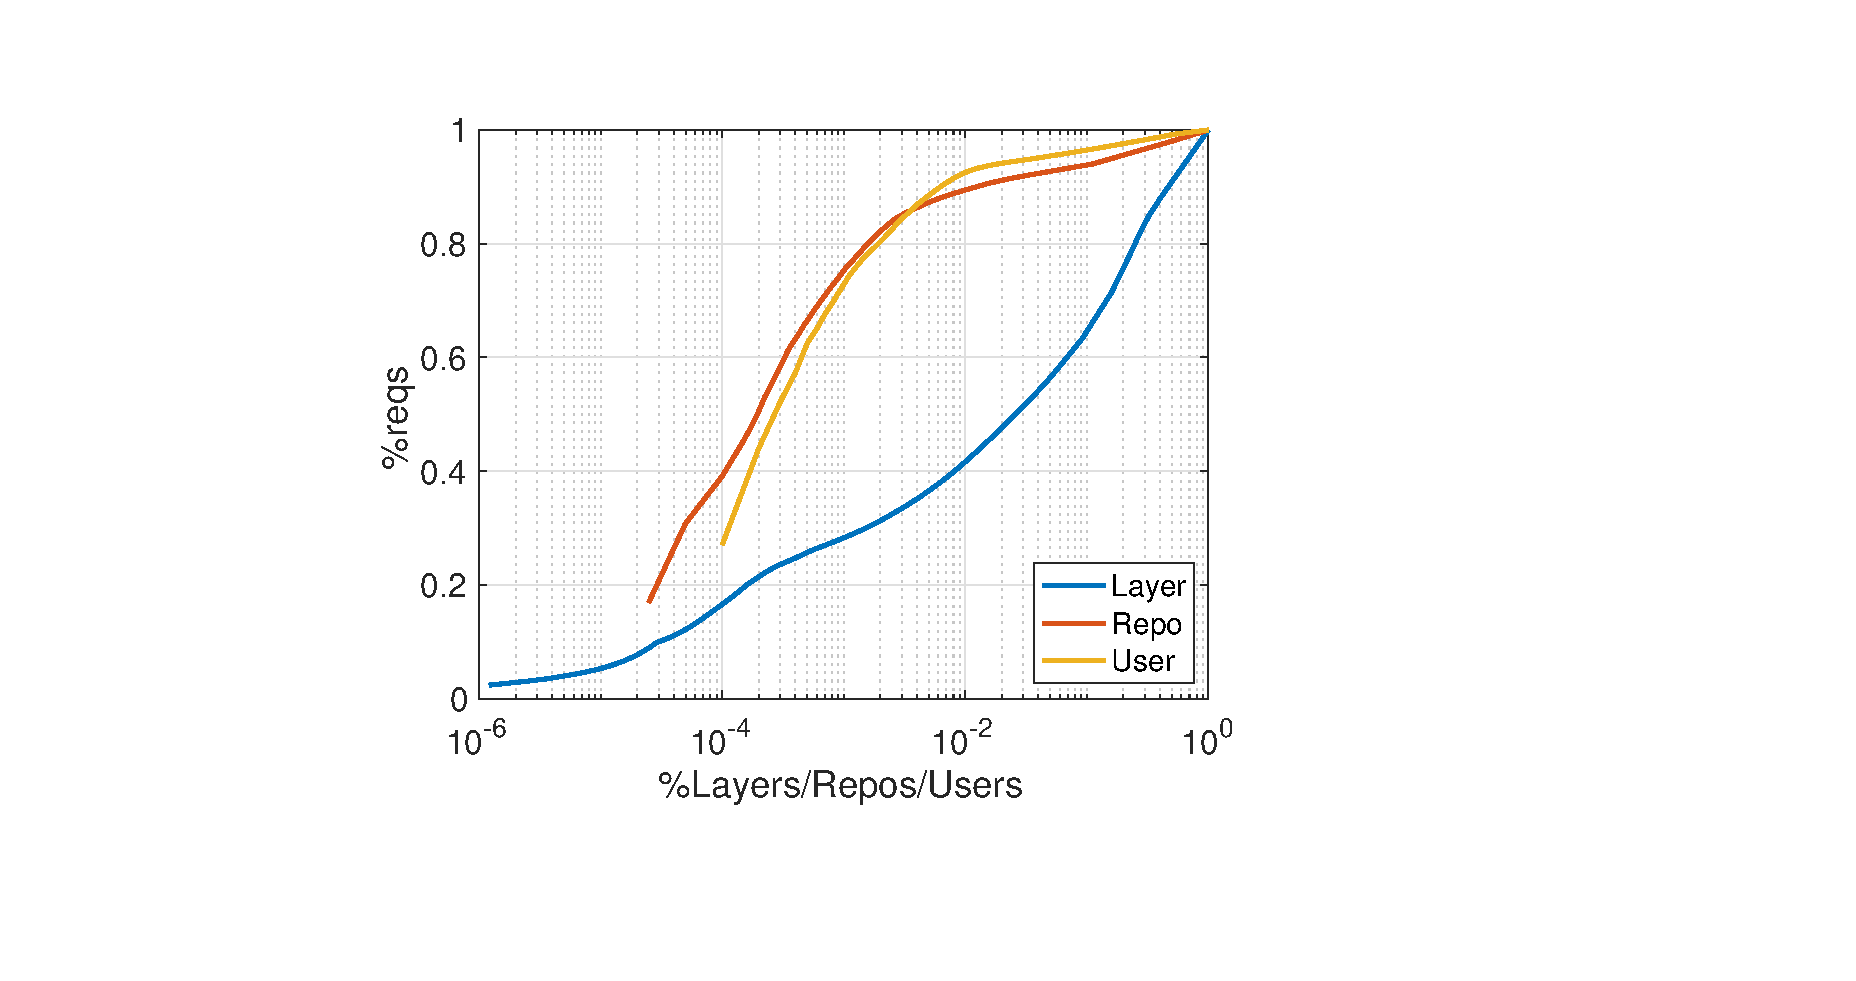
\includegraphics[width=1\textwidth]{graphs/skewness_cdf.eps}
			\caption{Popularity of layers, repos, and users.}
			\label{fig:sknewss}
		\end{minipage}
	\begin{minipage}{0.225\textwidth}
		\centering
		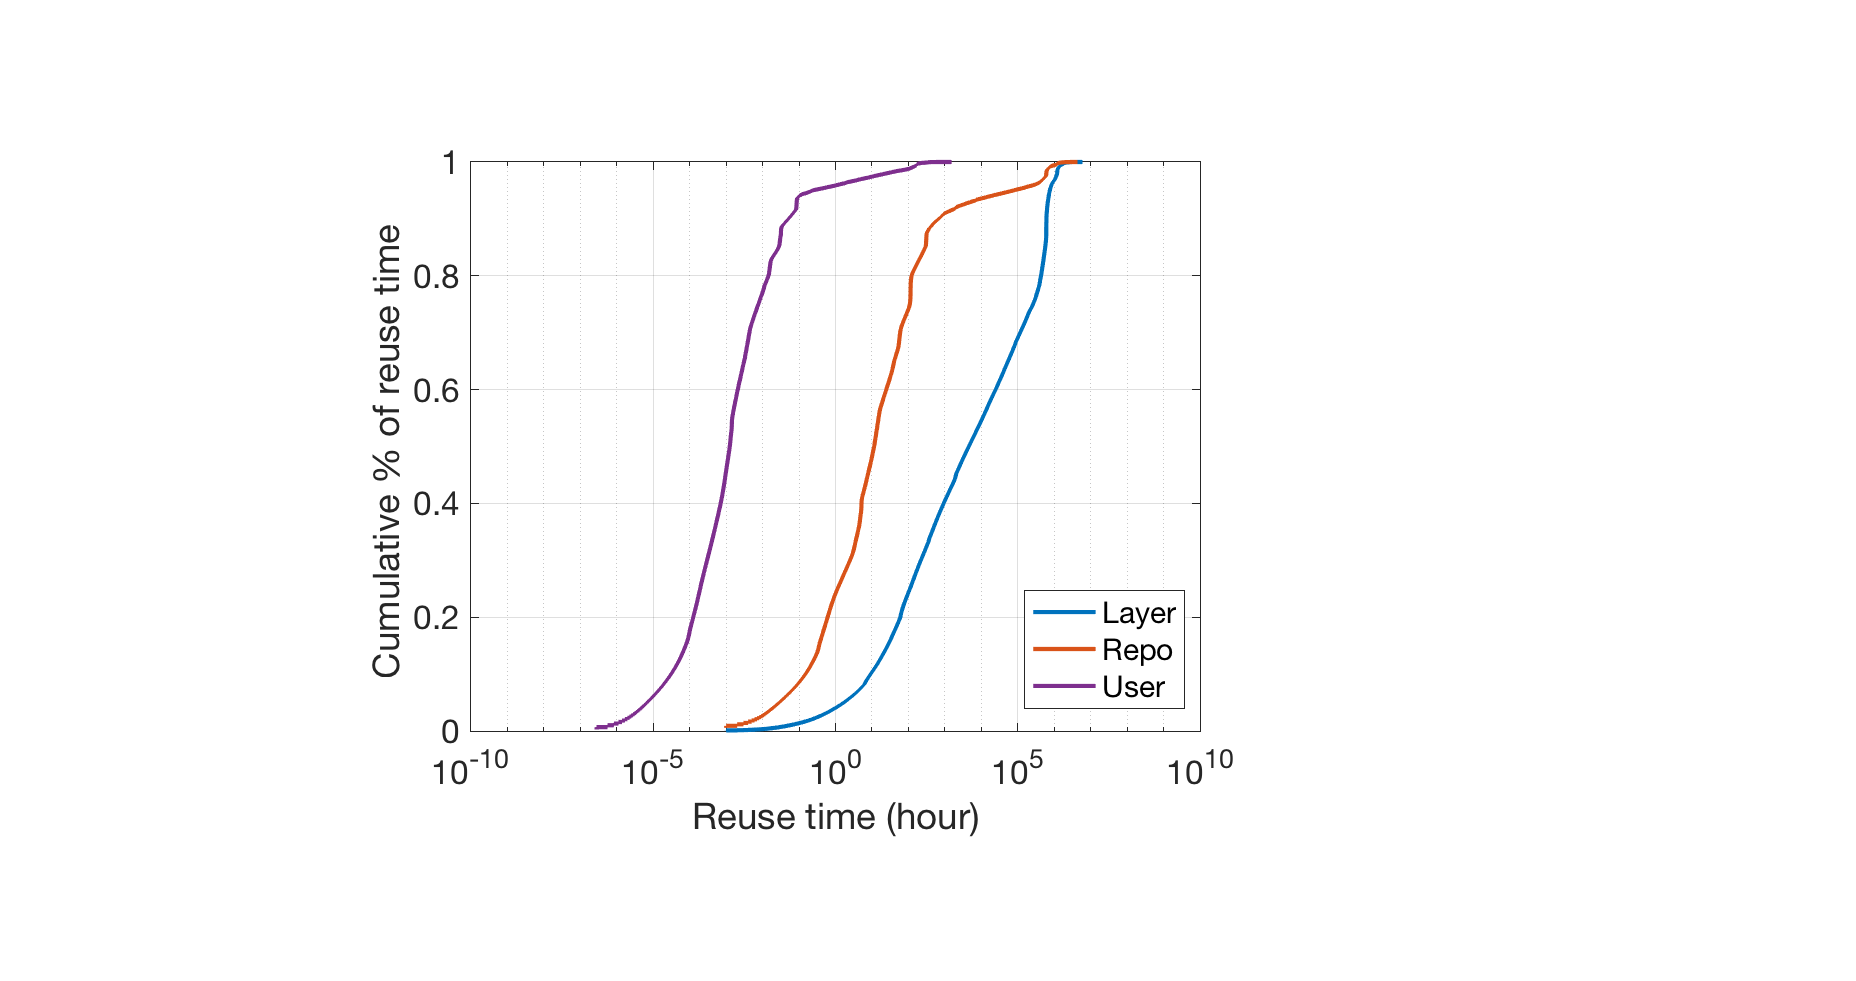
\includegraphics[width=1\textwidth]{graphs/reuse_time.eps}
		\caption{CDF of reuse time for layers, repos, and users.}
		\vspace{-3pt}
		\label{fig:reusetime}
	\end{minipage}
\end{figure}

The following observations are obtained by analyzing the Dallas(\texttt{dal}) registry workload collected from IBM Container Registry over the course of 75 days~\cite{dockerworkload}. 
\paragraph{Requests to layers are heavily skewed but layer reuse time is very long}

Figure~\ref{fig:sknewss} shows the registry accesses to layers and repositories, and accesses by users. 
Layer accesses are heavily skewed. For example, 25\% of popular layers account for 80\% of all requests. 
For repository accesses and accesses by users, the skew is more significant than it is for layers. %10\% most frequently accessed repositories account for 94\% of all requests
94\% of all requests are accessing only 10\% of the most frequently accessed repositories and only 9\% of users, most active ones, issued 97\% of all requests. 
This means that only a few extremely active users create their repositories in the \texttt{dal} registry and issue the majority of requests to the registry.

Figure~\ref{fig:reusetime} shows the reuse time of layers and repositories, and reuse time by users.
Reuse time is the duration between two subsequent requests to access the same layer or repository while 
the reuse time by user is defined as duration between two subsequent requests issued by the same user. 
The layer reuse time is long.
The median reuse time of a layer is 1.3 hours. 80\% of repositories experience the highest request frequency, with a reuse time of around 2 minutes. 
90\% of users remain active for at least 0.06 seconds.
%So for a registry, most of its stored layers are not accessed frequently given a very short time period while
%users can maintain active for a longer time. 
%This is because users can access multiple layers and manifests.
In other words, most of the layers stored in the
registry are not frequently requested in a very short
time period while users remain active for a longer time.
This is because users request different layers or manifests.

\paragraph{User active time is predictable} 
Based on the above observations, we believe that the user's active time is predictable. 
By just maintaining a LRU list of users, we achieved 99\% accuracy for predicting user active time.
For this reason, we utilize this predictability in our cache algorithm design.

